\TODO{Consider splitting in two chapters if they get too big}

While tiling itself is a well-known optimization technique, we most consider the parts of why it works.

\TODO{\dots}

\section{Theory}

In a sense, grouping columns is similar to striding clusters of data, except in the case when a row of work can't be perfectly strided.
When the width of a multidimensional array is not a multiple of the stride, the loads will not align column wise (\TODO{figure}).
To work around this, in the column approach we allow the last column to be narrower.

\begin{figure}[!hb]
    \centering
    
    \subfloat[Striding does not work well when the width of the task is a non-multiple of the striding factor.]{
        \centering
        \makebox[0.4\columnwidth][c]{
            \begin{tikzpicture}[scale=0.25, decoration = {
                markings, mark = between positions 0.3cm and 0.95 step 0.25cm with {\arrow{stealth}}
            }]
                \fill[gray]    (0, 3) rectangle +(4, 1);
                \fill[gray!50] (4, 3) rectangle +(4, 1);
                \fill[gray]    (8, 3) rectangle +(3, 1);

                \fill[gray]    (0, 2) rectangle +(1, 1);
                \fill[gray!50] (1, 2) rectangle +(4, 1);
                \fill[gray]    (5, 2) rectangle +(4, 1);
                \fill[gray!50] (9, 2) rectangle +(2, 1);

                \fill[gray!50] (0, 1) rectangle +(2, 1);
                \fill[gray]    (2, 1) rectangle +(4, 1);
                \fill[gray!50] (6, 1) rectangle +(4, 1);
                \fill[gray]    (10, 1) rectangle +(1, 1);

                \fill[gray]    (0, 0) rectangle +(3, 1);
                \fill[gray!50] (3, 0) rectangle +(4, 1);
                \fill[gray]    (7, 0) rectangle +(4, 1);

                \draw[step=1,gray!25] (0, 0) grid (11, 4);
            \end{tikzpicture}
        }
        \label{fig:striding_misalignment}
    }
    \qquad
    \subfloat[Allowing the last column to be flexible allows columns of thread groups to stay cohesive.]{
        \centering
        \makebox[0.4\columnwidth][c]{
            \begin{tikzpicture}[scale=0.25, decoration = {
                markings, mark = between positions 0.3cm and 0.95 step 0.25cm with {\arrow{stealth}}
            }]
                \fill[gray]    (0, 3) rectangle +(4, 1);
                \fill[gray!50] (4, 3) rectangle +(4, 1);
                \fill[gray]    (8, 3) rectangle +(3, 1);

                \fill[gray!50] (0, 2) rectangle +(4, 1);
                \fill[gray]    (4, 2) rectangle +(4, 1);
                \fill[gray!50] (8, 2) rectangle +(3, 1);

                \fill[gray]    (0, 1) rectangle +(4, 1);
                \fill[gray!50] (4, 1) rectangle +(4, 1);
                \fill[gray]    (8, 1) rectangle +(3, 1);

                \fill[gray!50] (0, 0) rectangle +(4, 1);
                \fill[gray]    (4, 0) rectangle +(4, 1);
                \fill[gray!50] (8, 0) rectangle +(3, 1);

                \draw[step=1,gray!25] (0, 0) grid (11, 4);
            \end{tikzpicture}
        }
        \label{fig:column_alignment}
    }
    \caption{
        \TODO{write this}
    }
    \label{fig:column_vs_striding}
\end{figure}

The index mapping $i \mapsto j$ to get the columning order consists out of four parts (figure \ref{fig:column_remap_parts}):
\begin{itemize}
    \item The starting offset of the column $o$.
    \item The column width $w'$.
    \item The index within a column $i'$
    \item The position within the column $(x, y)$
\end{itemize}

\begin{figure}[!hb]
    \centering
    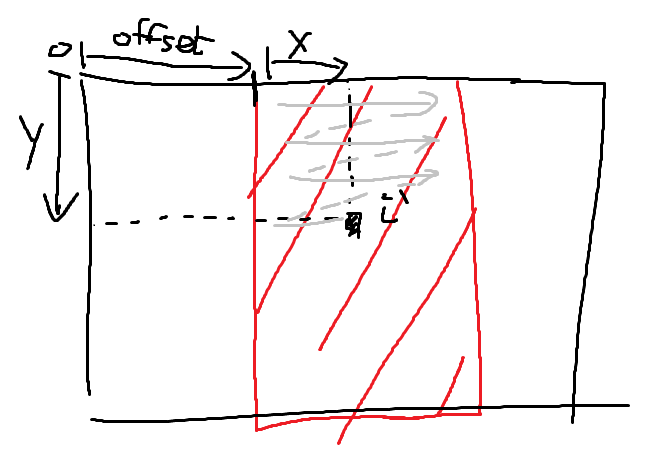
\includegraphics[width=8cm]{sketches/column_remap_parts.png}
    \caption{
        \TODO{aGKLJLKSG}
    }
    \label{fig:column_remap_parts}
\end{figure}


First, we calculate the offset for the starting index of the column we need to map to

\begin{align}
    o  &= \floor{\frac{i}{I_h w}} w
    \\ \intertext{Then, modify the width value such that the last column does not exceed the input width}
    w' &= \begin{cases}
        ((I_w - 1) \bmod w) + 1& \text{if last column}
        \\
        w & \text{otherwise}
    \end{cases}
    \\ \intertext{And take $i'$ as the index within a column}
    i' &= i \bmod I_h w'
    \\ \intertext{Calculate the position $(x, y)$ within the column}
    x & = i' \bmod w'
    \\ 
    y & = \floor{\frac{i'}{w'}}
    \\ \intertext{So that we can calculate $j$}
    \label{eq:column_mapping_to_j}
    j  &= x + y I_w + o
\end{align}

\TODO{should i add a figure showing the relation between the equation and the column pattern?}

\TODO{What are the effects of GPU warps (32 threads) with this schedule?}

On GPUs threads are batched in batches of 32 threads.
Therefore, increasing spatial locality between neighbouring threads can improve performance.

\subsection{Zigzagging variation}

A solution to increase thread locality within wraps in non-multiple widths of 32 is to zizzag on every other row.
We modify equation \ref{eq:column_mapping_to_j}
\begin{equation}
    j = \left(\begin{cases}
        x & y \text{ is uneven}
        \\
        w' - x & y \text{ is even}
    \end{cases}\right)  + y I_w + o
\end{equation}

\TODO{If we make columns fit for L2 cache, zigzagging may improve locality for lower level cache (L1) when columns sizes aren't a nice power of 2 (or)}

\subsection{Higher dimensions}

\section{Implementation in Accelerate}


\TODO{AAAAAAAAAAAA}


\begin{listing}[!ht]
    \begin{minted}{haskell}    
type ThreadMapping sh e arch 
    =  ShapeR sh 
    -> Operands sh 
    -> Operands Int 
    -> CodeGen arch (Operands Int)
    \end{minted}
    \label{lst:threadmapping_type}
\end{listing}

\begin{listing}
    \begin{minted}{haskell}
column :: Operands Int -> ThreadMapping sh e arch
column column_width shr sh index = do
    -- input sizes
    input_width  <- widthOp shr sh
    input_size   <- sizeOp  shr sh
    input_height <- input_size |//| input_width
    
    column_size  <- column_width |*|  input_height
    column_count <- ((input_size |+| column_size) |-| (1::Int)) |//| column_size

    column_index      <- index |//| column_size
    column_last_index <- column_count |-| (1::Int)
    column_offset     <- column_index |*| column_width

    index' <- index |%| column_size

    column_current_width <- ifThenElse (
        TupRsingle $ SingleScalarType $ NumSingleType (numType @Int), 
        column_index |==| column_last_index
      ) ( do
        input_width |-| (column_last_index |*| column_width)
      ) ( do
        return column_width
      )
    
    x_in_column <- index' |%|  column_current_width
    y_in_column <- index' |//| column_current_width
    result      <- x_in_column |+| (y_in_column |*| input_width) |+| column_offset

    return result
    \end{minted}
    \caption{
        \TODO{agaljhgal}
    }
    \label{lst:column_mapping}
\end{listing}

\begin{listing}
    \begin{minted}{haskell}
precomp_column :: Operands Int 
               -> ShapeR sh 
               -> Operands sh 
               -> CodeGen arch (Operands Int -> CodeGen arch (Operands Int))
precomp_column column_width shr sh = do
    -- input sizes
    input_width  <- widthOp shr sh
    input_size   <- sizeOp  shr sh
    input_height <- input_size |//| input_width
    
    column_size  <- column_width |*|  input_height
    column_count <- ((input_size |+| column_size) |-| (1::Int)) |//| column_size

    column_last_index <- column_count |-| (1::Int)

    return \index -> do
        column_index  <- index |//| column_size
        column_offset <- column_index |*| column_width
        index' <- index |%| column_size

        column_current_width <- ifThenElse (
            TupRsingle $ SingleScalarType $ NumSingleType (numType @Int), 
            column_index |==| column_last_index
        ) ( do
            input_width |-| (column_last_index |*| column_width)
        ) ( do
            return column_width
        )
        
        x_in_column <- index' |%|  column_current_width
        y_in_column <- index' |//| column_current_width
        result      <- x_in_column |+| (y_in_column |*| input_width) |+| column_offset

        return result
    \end{minted}
    \caption{
        The column mapping from listing \ref{lst:column_mapping} with precomputing the fixed parameters.
    }
    \label{lst:column_mapping_precompute}
\end{listing}

\section{Stencil Operation}

The naive stencil operations had problems of chasing the cache on sufficiently large input sizes which tiling does resolve (section \ref{sec:stencil_tiled}).
Consider what the tiling implies: we split the work on all axis, to improve locality.
However, all tiling except horizontal is unnecessary \TODO{bold claim, needs support} and may cause even more discontunuity in favourable access pattern.

Let us first consider the single threaded case of column based iteration: by controlling the column width we can force the ideal scenario of the naive stencil implementation (figure \ref{fig:stencil_naive_loading_pattern_ideal}) to occur, similarly to tiling.
The column based approach is similar to tiling, but also allows the ideal memory access pattern to continue accross tiles vertically.
In GPUs this translates to less cohesive threads as threadblocks get assigned in a round-robin fashion to SMs, eliminating posibilities of L1 cache reuse.

\begin{figure}[!hb]
    \centering
    
    \subfloat[Grouping by column only incurs a heavy load every time a new column is started.]{
        \centering
        \makebox[0.4\columnwidth][c]{
            \begin{tikzpicture}[scale=0.25, decoration = {
                markings, mark = between positions 0.3cm and 0.95 step 0.25cm with {\arrow{stealth}}
            }]
                \fill[gray!50]  (-1, -1) rectangle +(6, 4);
                \fill[gray!15] (3, 6) rectangle +(3, 3);

                \draw[step=1,gray!25] (-1, -1) grid (9, 9);

                \draw[gray, postaction = decorate] (0.5, 7.5) -- +(3, 0);
                \draw[gray, dashed] (3.5, 7.5) -- +(-3, -1);
                \draw[gray, postaction = decorate] (0.5, 6.5) -- +(3, 0);
                \draw[gray, dashed] (3.5, 6.5) -- +(-3, -1);
                \draw[gray, postaction = decorate] (0.5, 5.5) -- +(3, 0);
                \draw[gray, dashed] (3.5, 5.5) -- +(-3, -1);
                \draw[gray, postaction = decorate] (0.5, 4.5) -- +(3, 0);
                \draw[gray, dashed] (3.5, 4.5) -- +(-3, -1);
                \draw[gray, postaction = decorate] (0.5, 3.5) -- +(3, 0);
                \draw[gray, dashed] (3.5, 3.5) -- +(-3, -1);
                \draw[gray, postaction = decorate] (0.5, 2.5) -- +(3, 0);
                \draw[gray, dashed] (3.5, 2.5) -- +(-3, -1);
                \draw[black, postaction = decorate] (0.5, 1.5) -- +(3, 0);
                \draw[black, dashed] (3.5, 1.5) -- +(-3, -1);
                \draw[black, postaction = decorate] (0.5, 0.5) -- +(3, 0);

                \draw[black, dashed] (3.5, 0.5) -- +(1, 7);
                
                \draw[gray, postaction = decorate] (4.5, 7.5) -- +(3, 0);
                \draw[gray, dashed] (7.5, 7.5) -- +(-3, -1);
                \draw[gray, postaction = decorate] (4.5, 6.5) -- +(3, 0);
                \draw[gray, dashed] (7.5, 6.5) -- +(-3, -1);
                \draw[gray, postaction = decorate] (4.5, 5.5) -- +(3, 0);
                \draw[gray, dashed] (7.5, 5.5) -- +(-3, -1);
                \draw[gray, postaction = decorate] (4.5, 4.5) -- +(3, 0);
                \draw[gray, dashed] (7.5, 4.5) -- +(-3, -1);
                \draw[gray, postaction = decorate] (4.5, 3.5) -- +(3, 0);
                \draw[gray, dashed] (7.5, 3.5) -- +(-3, -1);
                \draw[gray, postaction = decorate] (4.5, 2.5) -- +(3, 0);
                \draw[gray, dashed] (7.5, 2.5) -- +(-3, -1);
                \draw[gray, postaction = decorate] (4.5, 1.5) -- +(3, 0);
                \draw[gray, dashed] (7.5, 1.5) -- +(-3, -1);
                \draw[gray, postaction = decorate] (4.5, 0.5) -- +(3, 0);
                \draw[red] (3,6) rectangle +(3, 3);
            \end{tikzpicture}
        }
    }
    \label{fig:}
    \qquad
    \subfloat[Tiling also incurs a heavy load when starting a new row of tiles, and due to having more rows also has more column starts.]{
        \centering
        \makebox[0.4\columnwidth][c]{
            \begin{tikzpicture}[scale=0.25, decoration = {
                markings, mark = between positions 0.3cm and 0.95 step 0.25cm with {\arrow{stealth}}
            }]
            \fill[gray!50] (3, 3) rectangle +(6, 4);
            \fill[gray!15] (-1, 2) rectangle +(3, 3);

            \draw[step=1,gray!25] (-1, -1) grid (9, 9);

            \draw[gray, postaction = decorate] (0.5, 7.5) -- +(3, 0);
            \draw[gray, dashed] (3.5, 7.5) -- +(-3, -1);
            \draw[gray, postaction = decorate] (0.5, 6.5) -- +(3, 0);
            \draw[gray, dashed] (3.5, 6.5) -- +(-3, -1);
            \draw[gray, postaction = decorate] (0.5, 5.5) -- +(3, 0);
            \draw[gray, dashed] (3.5, 5.5) -- +(-3, -1);
            \draw[gray, postaction = decorate] (0.5, 4.5) -- +(3, 0);
            \draw[gray, dashed] (3.5, 4.5) -- +(1, 3);
            \draw[gray, postaction = decorate] (4.5, 7.5) -- +(3, 0);
            \draw[gray, dashed] (7.5, 7.5) -- +(-3, -1);
            \draw[gray, postaction = decorate] (4.5, 6.5) -- +(3, 0);
            \draw[gray, dashed] (7.5, 6.5) -- +(-3, -1);
            \draw[black, postaction = decorate] (4.5, 5.5) -- +(3, 0);
            \draw[black, dashed] (7.5, 5.5) -- +(-3, -1);
            \draw[black, postaction = decorate] (4.5, 4.5) -- +(3, 0);
            
            \draw[black, dashed] (7.5, 4.5) -- +(-7, -1);

            \draw[gray, postaction = decorate] (0.5, 3.5) -- +(3, 0);
            \draw[gray, dashed] (3.5, 3.5) -- +(-3, -1);
            \draw[gray, postaction = decorate] (0.5, 2.5) -- +(3, 0);
            \draw[gray, dashed] (3.5, 2.5) -- +(-3, -1);
            \draw[gray, postaction = decorate] (0.5, 1.5) -- +(3, 0);
            \draw[gray, dashed] (3.5, 1.5) -- +(-3, -1);
            \draw[gray, postaction = decorate] (0.5, 0.5) -- +(3, 0);
            \draw[gray, dashed] (3.5, 0.5) -- +(1, 3);
            \draw[gray, postaction = decorate] (4.5, 3.5) -- +(3, 0);
            \draw[gray, dashed] (7.5, 3.5) -- +(-3, -1);
            \draw[gray, postaction = decorate] (4.5, 2.5) -- +(3, 0);
            \draw[gray, dashed] (7.5, 2.5) -- +(-3, -1);
            \draw[gray, postaction = decorate] (4.5, 1.5) -- +(3, 0);
            \draw[gray, dashed] (7.5, 1.5) -- +(-3, -1);
            \draw[gray, postaction = decorate] (4.5, 0.5) -- +(3, 0);
            \draw[red] (-1,2) rectangle +(3, 3);
            \end{tikzpicture}
        }
    }
    \caption{
        Visualisation of cache bottlenecks for both column based and tiling approaches. 
        \fsquare{red} Memory required by the next task.
        \fsquare{black} Tasks that still have their memory in cache.
        \fsquare{gray!50} Memory in cache.
        \fsquare{gray!15} Previous and upcoming tasks.
    }
    \label{fig:stencil_column_vs_tiling_pattern}
\end{figure}

The size of the cache needed $M_{size}$ can be approximated given the units per cache line $L$, column width $c$, stencil width $s_{w}$ and height $s_{h}$, and the number of active threads $t$. The required memory is independent of the size of the input data.

\[
    M_{size} = u \left(c + s_w\right) \left(s_h + \ceil{\frac{t}{c}}\right)
\]

Solving for $c$ gives an unneedly complex solution, so instead we approximate $M_{size}$ using the asymptote.

\[
    M_{size} = u \left(t + s_h \left(c + s_w\right)\right)
\]

Solving for column width $c$ gives 

\[
    c = \frac{M_{size} - u (s_h s_w + t)}{s_h u}
\]

\TODO{amount cache line fetches text here}
The amount of fetches is similar to equation \ref{eq:stencil_tiling_fetches}, however, since we do not divide the work horizontally anymore, the amount of cache line fetches is slightly less:

\begin{equation}
    F \leq \ceil{\frac{I_w}{c}}\ceil{\frac{c + S_w}{L}} (I_h + S_h)
    \label{eq:stencil_column_fetches}
\end{equation}

\TODO{Is a difference useful?}
\begin{equation}
    \Delta F \approx  
\end{equation}

\TODO{Calculate column parameters, spatial temporal diagrams}


\section{Matrix Multiplication}
Matrix multiplication may benefit from a column based approach due to many vertical reads.
Section \ref{sec:} \TODO{ref} showed that continuous vertical reads are more expensive than continuous horizontal reads (streaming).
Therefore, we want to keep data that is read vertically in cache for as long as possible.
The naive implementation (section \ref{sec:} \TODO{ref}) showed that working on an entire row of outputs requires to load the whole $I_w \times D$ data
By limiting the horizontal space we work on, we can control what stays in case, increasing reuse.


\begin{figure}
    \centering
    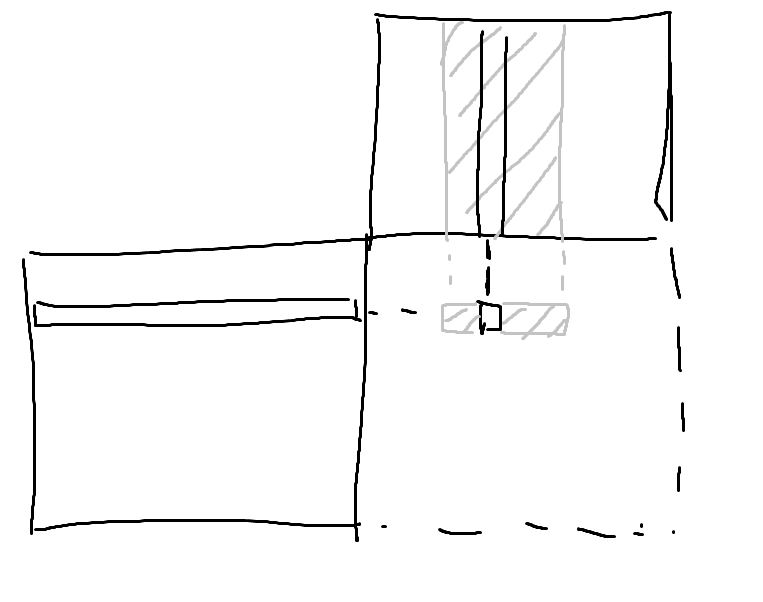
\includegraphics[width=8cm]{sketches/matrix_single_element_footprint.png}
    \label{fig:mm_cache_footprint}
    \caption{
        \TODO{asjlahkjg}
    }
\end{figure}

A matrix multiplication of $A \cdot B = C$ with $C$ being of size $I_w \times I_h$, and $A$ and $B$ being size $I_w \times D$ and $D \times I_h$ respectively, we compute the lower bound on the required cache by seperating the horizontal and vertical reads.




\[
    M_{l} = \ceil{\frac{d}{L}} + d\ceil{\frac{c}{L}}
\]

Similarly to stencil operations, approximate $M_{size}$ using the asymptote

\[
    M_{size} = u h c 
\]

Then solving for $c$

\[
    c = \frac{M_{size}}{u h}
\]

\TODO{Calculate column parameters, spatial temporal diagrams}
